% ============================================================
% GENERATED FILE -- DO NOT EDIT BY HAND.
% Produced by paper/icwsm/build_icwsm_source.py from paper/main.tex.
% Re-run that script after editing the journal source.
% ============================================================
\documentclass[letterpaper]{article}

% AAAI Author Kit 25. These style files are distributed by AAAI and are not
% redistributable, so they are not committed to this repository. Download the
% kit from https://aaai.org/authorkit25/ and place aaai25.sty (and companions)
% in this directory before building. See README.md.
\usepackage{aaai25}
\usepackage{times}
\usepackage{helvet}
\usepackage{courier}
\usepackage[hyphens]{url}
\usepackage{graphicx}
\usepackage{natbib}
\usepackage{booktabs}
\usepackage{amsmath, amssymb}
\usepackage{placeins}
\usepackage{float}
\usepackage[caption=false]{subfig}
\urlstyle{rm}
\def\UrlFont{\rm}
\frenchspacing
\setlength{\pdfpagewidth}{8.5in}
\setlength{\pdfpageheight}{11in}

\pdfinfo{
/TemplateVersion (2025.1)
}

\setcounter{secnumdepth}{0}

\title{Who Turns to AI for Schoolwork? \\
Socioeconomic and Educational Predictors of Student Interest in the ChatGPT Era}

% ICWSM 2027 uses double-anonymous review. Author and affiliation are
% suppressed for submission and restored for the camera-ready version.
\author{}
\affiliations{}

\begin{document}
\maketitle


% ==========================================================
\begin{abstract}
\noindent
Since ChatGPT's release in late 2022, adoption of generative AI by students has been rapid but uneven. This study links regional socioeconomic and educational conditions before ChatGPT’s release to subsequent student-oriented interest in using AI for schoolwork. Using Google Trends search interest across 73 student-intent keywords (2023--2025) at the Designated Market Area (DMA) level and a pre-ChatGPT 2019 snapshot built from American Community Survey and Stanford Education Data Archive records, we find that smaller, less affluent DMAs with lower degree attainment show the highest subsequent interest in AI for schoolwork. A gradient boosting model trained on seven 2019 features explains roughly 39\% of cross-DMA variance in 2023--2025 search interest under repeated cross-validation. A five-cluster regional typology places a non-metropolitan Southern cluster with markedly elevated Black population shares at the top of the interest ranking and Hispanic-majority Southwestern metros third, though racial composition is not itself an independent predictor once attainment and income are accounted for. The pattern is counterintuitive relative to the documented regional divide in general-purpose ChatGPT awareness and search interest, and it converges with newer student-level survey evidence showing elevated schoolwork-related AI use among Black and Hispanic teens. The findings suggest that student interest in AI for schoolwork may track structural inequity rather than simple early-adopter advantage. This has direct implications for how schools design AI academic-integrity policies: punitive enforcement regimes will fall hardest on the lower-income, lower-attainment communities where schoolwork-related AI demand appears highest, and, on the survey and discipline-disparity evidence, disproportionately on Black and Hispanic students within them. We argue that student AI interest is best treated as symptomatic of resource gaps, not as misconduct to be policed.
\end{abstract}

\noindent\textbf{Keywords:} generative AI; education; digital divide; Google Trends; academic integrity; ChatGPT.

% ==========================================================
\section{Introduction}

Since the release of ChatGPT in late 2022, the U.S. education system has been grappling with rapid student uptake of generative AI. By 2025, 70\% of U.S.\ high school students reported using generative AI in some form~\citep{laird2025}, and roughly 11\% of student writing since 2023 has contained at least 20\% AI-generated content by one major academic-integrity platform's estimate~\citep{turnitin2024}. School responses have ranged from outright bans to AI-integration pilots, and most teachers report receiving no guidance at all on AI use in class~\citep{laird2025}.

Research on the population-level distribution of generative AI has so far focused heavily on general-purpose AI awareness and adoption. \citet{daepp2025} show that U.S.\ regions with higher ChatGPT search interest are more educated and economically advantaged, suggesting a familiar digital-divide pattern in early generative AI awareness. Student-focused evidence, however, complicates that pattern: recent surveys show that Black and Hispanic teens report higher rates of schoolwork-related chatbot use than White teens, even as higher-income students may have greater awareness of particular tools and greater capacity to convert AI use into academic benefit~\citep{sidoti2025, pew2026}. General-audience AI searches therefore conflate multiple populations and multiple mechanisms---professional use, casual experimentation, student help-seeking, and academic shortcutting. What remains underexplored is whether regional student-intent search interest for schoolwork-related AI follows the same geography as generic ChatGPT interest.

This paper asks: \emph{what socioeconomic and educational conditions in a U.S.\ region in 2019 predict its students' interest in using generative AI for schoolwork in 2023--2025?} The unit of analysis is the Designated Market Area (DMA), the Nielsen-defined regional grouping at which Google Trends exposes search-interest data~\citep{nielsen2025}. The framing deliberately ties a pre-ChatGPT ``snapshot'' to post-ChatGPT interest. We use 2019 conditions rather than a 2023--2025 cross-sectional design for three reasons. First, 2019 conditions cannot have been caused by post-2022 AI search behavior, ruling out reverse causality at the level of the predictors. Second, 2019 reflects the structural pre-AI educational and economic landscape; using contemporaneous conditions would conflate pre-existing inequality with pandemic disruption, post-pandemic recovery, and any AI-induced changes (e.g., school AI policy adoption, AI-related shifts in employment). Third, 2019 is the last fully pre-COVID, pre-ChatGPT school year for which county-level achievement data are unambiguously a baseline. The design therefore lets us ask whether student AI interest is tracking prior \emph{advantage} (a fast-followers story in which the resource-rich first adopt new technology) or prior \emph{disadvantage} (an access-seeking story in which students turn to AI precisely where schools or households are under-resourced).

We find the latter. The result holds across multiple methods (OLS, Lasso, bootstrap Lasso, an unsupervised k-means typology, supervised gradient boosting regression). Regions that in 2019 were smaller, poorer, and less educated show the highest 2023--2025 student AI-for-schoolwork search interest. Racial composition enters this picture at the level of the regional typology rather than as an independent marginal effect: the highest-interest cluster is a non-metropolitan Southern group with markedly elevated Black population shares, but neither Black nor Hispanic share is a significant predictor in the supervised feature set once attainment and income are held constant. Seven 2019 features explain about 39\% of the cross-region variance in that interest under repeated cross-validation.

The paper's contributions are:
\begin{itemize}
    \item A cross-sectional, DMA-level dataset linking 2019 pre-ChatGPT socioeconomic and educational conditions to 2023--2025 student-intent AI search interest, assembled from Google Trends, the American Community Survey, and the Stanford Education Data Archive (SEDA).
    \item An adaptation of the anchor-bank principle of \citet{west2020} to a 19-batch student-intent keyword design at the DMA level, allowing many low-volume student-intent terms to be placed on a common scale despite the Google Trends API's relative-only volume reporting.
    \item Evidence that pre-existing socioeconomic and educational disadvantage predicts higher regional student-intent AI-for-schoolwork search interest, a pattern that diverges from the geography of general-purpose ChatGPT search interest and whose highest-interest regional cluster converges with newer survey evidence on schoolwork-related chatbot use among Black and Hispanic teens.
    \item A policy proposition: if interest signals access-seeking, then punitive AI policies in schools will disproportionately harm the communities whose students have the strongest motivation to use the technology.
\end{itemize}

% ==========================================================
\section{Related Work}

\paragraph{Generative AI and the digital divide.}
Research on generative AI adoption increasingly shows that access to, awareness of, and benefit from AI tools are socially patterned. \citet{daepp2025} provide the closest regional analogue to the present study. Using Google Trends search data, they show that U.S.\ counties with higher ChatGPT search interest were more urban, higher income, more educated, more Asian, and more concentrated in technology-related employment, with educational attainment emerging as the strongest predictor in adjusted models. Survey evidence in higher education points the same way: the 2025 Higher Education Policy Institute student survey reports a ``growing digital divide in AI use,'' with more socioeconomically advantaged students more likely to report using generative AI tools for academic work~\citep{hepi2025}. This finding is consistent with classic first-level and second-level digital-divide accounts, in which advantaged people and places tend to encounter new technologies earlier and are better positioned to convert access into effective use and downstream benefits~\citep{vandijk2005, hargittai2002}. Yet generative AI also differs from older educational technologies. Many GenAI tools are free or low-cost, mobile-accessible, and capable of providing individualized writing, translation, explanation, and tutoring support. As a result, the distribution of general AI awareness need not match the distribution of student demand for schoolwork support. The present study builds from this tension by asking whether pre-ChatGPT regional advantage predicts later student-intent AI search interest, or whether schoolwork-related interest instead concentrates in regions marked by prior educational and socioeconomic disadvantage.

\paragraph{Student AI use and educational inequality.}
Student-focused evidence complicates a simple ``advantaged-first'' adoption story. Survey research shows rapid growth in AI use for schoolwork among U.S.\ teens. The Pew Research Center reported that the share of teens using ChatGPT for schoolwork doubled from 13\% in 2023 to 26\% in 2024, with Black and Hispanic teens reporting higher schoolwork use than White teens in the 2024 survey~\citep{sidoti2025}. More recent Pew evidence on chatbots broadly shows a similar pattern: Black and Hispanic teens are more likely than White teens to report using chatbots for schoolwork, to find them helpful, and to say they complete all or most of their schoolwork with chatbot help~\citep{pew2026}. These survey findings suggest that student AI use may reflect not only privileged early adoption, but also compensatory demand for academic support.

Research in higher education likewise suggests that AI inequality is multidimensional. \citet{zhang2025} find that socioeconomic status, gender, race/ethnicity, and adoption experience are associated with U.S.\ college students' perceived acceptability and educational benefits of ChatGPT. \citet{zhang2026} further distinguish general digital literacy from AI literacy, showing that socioeconomic status is more strongly associated with AI literacy than with general digital literacy and that students' ChatGPT activities can be separated into academic-support and displacement uses. \citet{beckman2025} similarly argue that a GenAI divide may emerge through unequal access, unequal capabilities, and unequal capacity to convert AI use into educational advantage. Large-scale behavioral evidence points in the same direction. \citet{yu2024} analyze more than one million college writing submissions and find post-ChatGPT improvements in writing quality, but with uneven equity implications---some linguistic gaps narrowed, while equitizing benefits were more concentrated among students from higher-socioeconomic-status households. Together, this literature suggests that AI use, AI literacy, and AI benefit should not be treated as interchangeable outcomes.

\paragraph{Contribution of the present study.}
Existing student-focused work is primarily survey-based, institution-specific, or based on observed student submissions within particular learning platforms. Existing regional search-based work, by contrast, generally measures generic ChatGPT or AI interest, which mixes students with professionals, software workers, casual users, parents, and other populations. The present study connects these literatures by isolating a student-intent, schoolwork-related search signal at the Designated Market Area level and linking it to pre-ChatGPT socioeconomic and educational conditions. The contribution is therefore not the first evidence that student AI use varies by demographic group, but rather a regional, pre--post design showing that schoolwork-related AI interest has a different socioeconomic geography from general ChatGPT search interest.

\paragraph{Academic integrity, AI detection, and unequal enforcement risk.}
The distribution of student AI interest matters because schools often respond to generative AI through academic-integrity policies, restrictions, and detection tools~\citep{laird2025}. Yet AI-detection tools raise substantial fairness and reliability concerns. \citet{liang2023} show that GPT detectors frequently misclassify writing by non-native English writers as AI-generated, a pattern the authors attribute to detectors treating lower lexical and syntactic variability as AI-like. Policy research has likewise argued that AI-detector use can disproportionately affect English learners, and broader school-discipline research documents persistent racial disparities in punitive educational sanctions~\citep{woelfel2023, darlinghammond2024}. These findings do not imply that all AI use is educationally beneficial, nor that schools should ignore academic integrity. They do imply that enforcement-centered responses can reproduce existing inequities when the students most likely to seek AI assistance are also students most exposed to unequal disciplinary systems.

\paragraph{Google Trends as a regional signal.}
Google Trends has been used as a proxy for public attention across domains including epidemiology, political issue salience, and technology diffusion~\citep{choi2012, mellon2014, jun2018}. Its strengths are geographic coverage, timeliness, and the ability to observe interest in emerging behaviors before administrative data exist. Its limitations are equally important. Google Trends returns normalized relative search interest rather than absolute search volume, and Google cautions that Trends is not a scientific poll and should be interpreted as one signal among others~\citep{googletrends}. Recent methodological reviews warn that many social-science applications of Google Trends under-test internal validity, reliability across pulls, and generalizability~\citep{holzl2025}. These concerns are especially relevant for low-volume keywords and small geographies. Because Google Trends scales each query batch internally and limits comparison sets, multi-keyword designs require calibration. \citet{west2020} formalizes an anchor-bank strategy for placing many Trends series on a common scale. The present study uses the same general principle, repeatedly querying target terms with a shared high-volume anchor term to compare student-intent keywords across batches. The DMA resolution covers the continental U.S.\ and parts of Hawaii and Alaska~\citep{nielsen2025}.

\paragraph{Regional education data and the pre-ChatGPT baseline.}
The Stanford Education Data Archive (SEDA) provides nationally comparable achievement measures linked to U.S.\ educational and census geographies. SEDA releases include district- and county-level achievement measures, subgroup estimates, and covariates, with newer releases extending beyond the version used here~\citep{reardon2025}. Later SEDA-related recovery releases are valuable for studying pandemic recovery, but they are conceptually different from the pre-treatment baseline required for this design.

% ==========================================================
\section{Data}
\label{sec:data}

We assemble one cross-sectional dataset of 209 U.S.\ Designated Market Areas (DMAs). We use DMAs as the unit of analysis because Google Trends provides geography-specific relative-interest data at this resolution, while smaller geographies are more vulnerable to low-volume suppression and instability.

\subsection{Student AI-for-schoolwork interest}

We use Google Trends (via the open-source \texttt{pytrends} library~\citep{pytrends2023}) to measure regional interest, with timeframe 2023-01-01 through 2025-07-31 and geographic resolution \texttt{DMA}.

\paragraph{Keyword selection.}
After exploratory querying through the Google Trends web interface, we selected 73 keywords specific to student AI use for schoolwork. Keywords span eight conceptual groupings: practical homework help, specific AI tools (e.g., PhotoMath, Khanmigo, Socratic), AI techniques (e.g., prompt engineering), AI writing support, subject-specific help, exam preparation, accuracy and hallucination, and plagiarism / detection policy. We excluded generic terms such as ``AI,'' ``ChatGPT,'' or ``Gemini'' because they capture non-student traffic. The full keyword list appears in Appendix~A.

\paragraph{Anchored batching.}
Google Trends returns relative interest on a 0--100 scale within each query batch~\citep{googletrends}, with at most five keywords per batch~\citep{googletrends_api_2025}. Values are therefore not directly comparable across batches. We use an \emph{anchor-normalization} strategy, building on the anchor-bank principle of \citet{west2020}: every batch includes the high-volume term ``homework'' as a fifth keyword, and its per-DMA score serves as a common scale. Concretely, for each (DMA, keyword) pair we scale the raw score by the ratio of the DMA's median anchor score across all batches to the anchor score in the keyword's own batch, then average over batches. The 73 target keywords are distributed across 19 batches: 18 full batches each consisting of the anchor plus four target keywords, and one final partial batch consisting of the anchor plus one target keyword (\texttt{AI tutor app}). Batches are hard-coded for reproducibility (see code release).

\paragraph{Per-DMA interest score.}
We average the anchor-normalized per-keyword scores within each DMA to obtain a single scalar, \texttt{search\_interest}, representing the DMA's overall student AI-for-schoolwork search interest over 2023--2025.

\paragraph{Interpreting the outcome.}
Google Trends reports normalized relative search interest rather than absolute search volume. Each value is computed as the share of all searches in the geography and time range that match the query, then re-scaled to 0--100 within the comparison batch~\citep{googletrends}. The outcome is therefore a per-capita-style relative measure, not an absolute volume measure: a small DMA in which a large fraction of searches are about AI for schoolwork will register a higher value than a large DMA in which a small fraction are. This is exactly the interpretation we want, since regional claims of the form ``smaller DMAs show higher interest'' are claims about per-capita propensity, not about absolute query counts. The anchor-normalized score makes keyword batches comparable but does not recover absolute query volume. In robustness checks, we therefore treat the outcome as an information-seeking signal and test sensitivity to keyword families, especially academic-integrity and detector-related terms that may reflect concern about enforcement rather than direct use of AI tools.

\paragraph{Missingness and the analytic sample.}
Google Trends returns \texttt{NaN} when a keyword's volume falls below an unspecified reporting threshold in a given region~\citep{googletrends}. The Trends outcome is pulled directly at DMA resolution and is not aggregated from any sub-DMA geography; it is the ACS and SEDA covariates that are aggregated up from county to DMA. After anchor normalization within and across batches and merging with the county-to-DMA-aggregated ACS and SEDA covariates, eleven low-population DMAs (Alpena MI, Glendive MT, Helena MT, Juneau AK, North Platte NE, Presque Isle ME, Zanesville OH, Fairbanks AK, Mankato MN, Ottumwa IA-Kirksville MO, and St.\ Joseph MO) have no observed search-interest value.

Google documents \texttt{NaN} as indicating volume that is either unavailable or below an unspecified reporting threshold, and it does not distinguish the two cases. Neither available treatment is therefore assumption-free, and the two err in opposite directions. Excluding these DMAs is the conventional complete-case choice and avoids assigning a fabricated value to the dependent variable~\citep{vonhippel2007}, but the missingness is not ignorable. These regions are unobserved precisely because their search volume was low, and they are small and rural, which is the profile our results in Section~\ref{sec:results} associate with \emph{higher} interest. Excluding them may therefore flatter the reported gradient. Coding them at zero instead treats ``unmeasurably small'' as ``lowest possible interest,'' which is a strong assumption, but a conservative one. Zero lies below the lowest observed value in the data, so this coding attenuates the gradient rather than inflating it.

Because neither treatment is clearly correct, we adopt the complete-case sample of 198 DMAs as the primary analytic sample and report the zero-coded 209-DMA sample alongside it throughout. Appendix~\ref{sec:approbust} reports both, together with two further sensitivity checks. The cluster ordering in Section~\ref{sec:results} is the same under both treatments, as are the direction and significance of every predictor gradient we report.

\subsection{Socioeconomic snapshot (ACS 2019)}

For the pre-ChatGPT snapshot, we pull the U.S.\ Census Bureau's American Community Survey (ACS) 5-year estimates for 2015--2019 at the county level~\citep{acs2019}. The ACS 5-year product pools sample data collected from 2015 through 2019 into a single estimate published in 2020, providing reliable measurement for small geographies that the 1-year product cannot cover (the 1-year product is only published for counties with population above 65{,}000). It is therefore not an average of five separate annual datasets, but a single 2015--2019 estimate centered on conditions immediately before the COVID and ChatGPT shocks.

From ACS we extract median household income, poverty count and denominator (table B17001), population (B01003), educational attainment (B15003), and racial composition using the mutually-exclusive categories of table B03002. We engineer three rates: \texttt{poverty\_rate}, \texttt{bach\_plus\_rate} (share of adults with a bachelor's degree or higher), and \texttt{grad\_prof\_rate} (share with master's, professional, or doctoral).

\paragraph{Choice of racial-ethnic categories.}
We use ACS table B03002 (Hispanic or Latino origin by race) rather than B02001 (Race alone) because B03002 separates Hispanic/Latino ethnicity from race and yields a set of mutually exclusive Hispanic and non-Hispanic-by-race groupings (in this paper: Hispanic, non-Hispanic white, non-Hispanic Black, non-Hispanic Asian). These categories are administrative constructs, defined by OMB Statistical Policy Directive No.\ 15 and operationalized by the Census Bureau; we do not treat them as biological or as a substantively well-defined partition of human variation. We use them for two reasons. First, B03002 is the categorical scheme under which the federal data infrastructure (Census, ACS, NCES, SEDA) and the contemporary inequality and education-policy literature report population shares, so analyzing DMA composition in these categories is necessary to merge with SEDA and to compare against existing work. Second, the survey evidence on student AI use that motivates this paper is itself reported in the same Hispanic, non-Hispanic Black, non-Hispanic Asian, non-Hispanic white scheme~\citep{sidoti2025,pew2026}; using B03002 keeps the regional analysis interpretable in the same vocabulary as the survey results we compare it to. The choice therefore reproduces the categorical boundaries imposed by federal statistical practice; the alternative---an internally constructed grouping---would gain conceptual cleanliness at the cost of comparability with both the data sources and the literature this paper engages.

\subsection{Educational achievement (SEDA 2019)}

Regional student achievement comes from the Stanford Education Data Archive, filtered to the 2018--2019 school year~\citep{reardon2025}; the baseline rationale is given in the Introduction. SEDA provides nationally comparable achievement measures linked to U.S.\ educational and census geographies. We retain only the high-level aggregates with zero missingness at the county level---overall mean ELA and math scores---plus grade-specific scores for grades 3--8 (used only in a multicollinearity check, not in the main model).

\subsection{Geographic merge}

County records from ACS and SEDA are aggregated to the DMA level using a publicly available FIPS-to-DMA crosswalk~\citep{kapastor2021}. For rates we compute population-weighted means, and for counts we sum. After merging with the Google Trends scores, the full analytic frame contains 209 DMAs with complete predictor information, of which 198 have observed search-interest outcomes. The primary models use those 198; the remaining 11 enter only through the zero-coded sample reported alongside. Table~\ref{tab:vars} in Appendix~\ref{sec:appdata} lists all variables.

% ==========================================================
\section{Methods}

Our pipeline moves from broad feature space to a parsimonious predictive model in three stages.

\subsection{Feature selection}

We begin with a standardized OLS regression with mean imputation on a 14-feature set: nine ACS demographic and economic features and five high-level SEDA achievement features (overall ELA, overall math, and three subject-level grade-aggregate scores). Grade-level SEDA scores are excluded from the OLS feature set because they sum mechanically to the overall score. Racial proportions remain in the feature set despite summing to approximately 100\%, since dropping any single share would discard interpretable information.

To stabilize selection under collinearity, we use Lasso with cross-validated penalty (\texttt{LassoCV}, 5-fold). Because a single Lasso fit is sensitive to correlated predictors, we additionally run a bootstrap Lasso with 1000 resamples and report, for each feature, its coefficient at the full-sample fit, its selection probability across bootstrap iterations, and its 95\% bootstrap confidence interval.

From the convergence of OLS coefficients, Lasso coefficients, and bootstrap selection probability, we identify a candidate set consisting of income, poverty, educational attainment, population, racial composition, and overall ELA achievement. Because several of these variables are strongly collinear (notably the racial-composition shares and income/poverty/education), we use two parsimonious feature subsets at later stages---one for clustering and one for the supervised predictor---chosen to keep each model identifiable while remaining faithful to the candidate set. The two subsets overlap but are not identical, and we describe them explicitly below. Poverty rate, graduate/professional rate, and several variables outside each subset are retained for sensitivity checks.

\subsection{Typology via k-means clustering}

We cluster DMAs over seven standardized features: \texttt{bach\_plus\_rate}, \texttt{score\_all\_ela}, \texttt{pct\_nh\_black}, \texttt{median\_income}, \texttt{pct\_hispanic}, \texttt{pct\_nh\_asian}, and \texttt{pct\_nh\_white}. These are chosen to capture educational, racial, and income structure while avoiding the large dynamic range of population, which dominates a Euclidean clustering when included. We sweep $k \in \{1, \ldots, 50\}$ and select $k$ using within-cluster sum of squares (elbow), mean inter-centroid distance, and silhouette score; all three diagnostics agree on $k=5$. Missing overall ELA scores for nine DMAs are imputed by averaging the ten nearest neighbors in the standardized predictor space.

Cluster assignments are then plotted geographically. DMA names differ between the Trends data and the reference GeoJSON~\citep{simzou}, so we perform fuzzy string matching with a similarity threshold of 80.

\subsection{Predictive model}

To assess how much of the variance in 2023--2025 AI-for-schoolwork interest is attributable to 2019 conditions, we train supervised regressors to predict \texttt{search\_interest}. The headline supervised model uses a parsimonious seven-feature set---\texttt{median\_income}, \texttt{bach\_plus\_rate}, \texttt{population}, \texttt{pct\_hispanic}, \texttt{pct\_nh\_black}, \texttt{pct\_nh\_asian}, and \texttt{score\_all\_ela}---chosen to retain population (which contributes substantial variance to the supervised target despite being deliberately excluded from clustering) while dropping \texttt{pct\_nh\_white} to reduce collinearity with the other racial-composition shares. The supervised seven-feature set therefore differs from the clustering seven-feature set by swapping \texttt{pct\_nh\_white} for \texttt{population}; this distinction matters and we keep it explicit throughout.

We evaluate Linear, Ridge, Lasso, Random Forest, and Gradient Boosting under repeated cross-validation with \texttt{random\_state=42}. Linear, Ridge, and Lasso converge to roughly equivalent performance ($R^2 \approx 0.15$), while Random Forest and Gradient Boosting both produce a substantially higher $R^2$ in the range $0.39$ to $0.42$. The two tree ensembles are close in mean performance, with the untuned Random Forest marginally ahead, but the tuned Gradient Boosting model is markedly more stable across fold assignments. We therefore select tuned Gradient Boosting as the headline model on the basis of stability rather than mean alone, and use a grid search over \texttt{n\_estimators}, \texttt{learning\_rate}, \texttt{max\_depth}, and \texttt{min\_samples\_split} (with 5-fold CV inside the search) to fix its hyperparameters, then report mean $\pm$ SD of $R^2$ across 10 repetitions of an outer 5-fold cross-validation. The full comparison is reported in Section~\ref{sec:supervised}; the linear and tree-ensemble families agree qualitatively on which features matter most, but disagree by more than a factor of two on $R^2$, which is the basis for selecting the tree-ensemble family for the headline. Poverty rate, graduate/professional rate, and \texttt{pct\_nh\_white} are retained for sensitivity checks but excluded from the headline model to reduce redundancy.

% ==========================================================
\section{Results}
\label{sec:results}

\subsection{Univariate relationships}

Figure~\ref{fig:lowess} plots search interest against each of the three socioeconomic-attainment predictors with a LOWESS smoother. As 2019 DMA median income, bachelor-plus rate, and graduate-attainment rate rise, 2023--2025 AI-for-schoolwork search interest falls. These directions persist through all subsequent analyses.

\begin{figure}[!htbp]
\centering
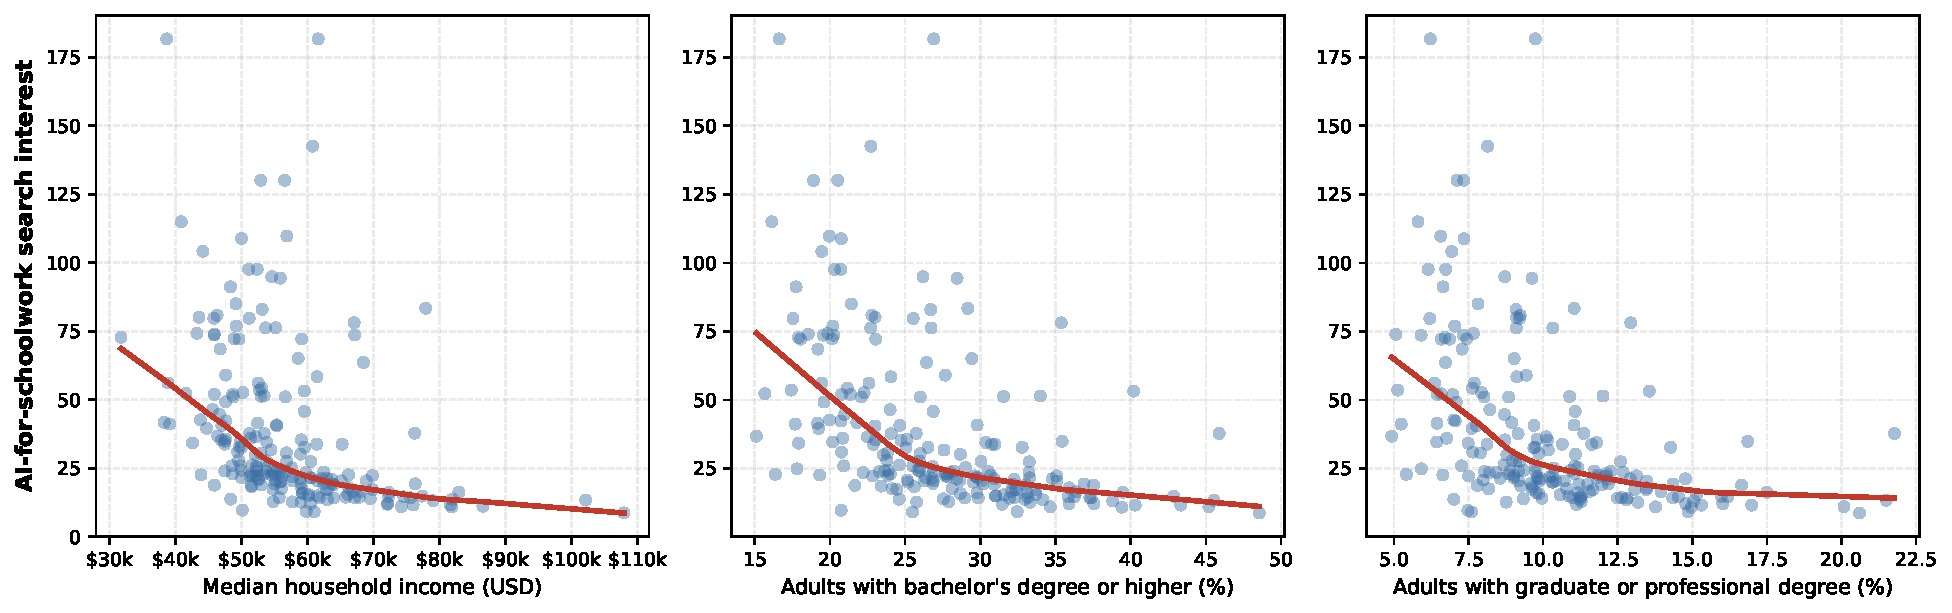
\includegraphics[width=\linewidth]{../figures/fig_lowess.pdf}
\caption{LOWESS relationships between 2019 DMA characteristics and 2023--2025 AI-for-schoolwork search interest, for three socioeconomic-attainment predictors. As 2019 median household income, bachelor-plus rate, and graduate/professional attainment rise, AI-for-schoolwork search interest falls.}
\label{fig:lowess}
\end{figure}

\FloatBarrier
\subsection{Convergent feature selection}

Across the feature-selection stages (standardized OLS, LassoCV, and bootstrap Lasso with 1000 resamples), four feature groups are consistently retained: educational attainment (bachelor-plus rate), racial composition (Asian, Hispanic, and Black shares), population size, and income. Selection probability under bootstrap Lasso is highest for the bachelor-plus rate, which we therefore characterize as the single most \emph{stably selected} predictor across resamples. This is a statement about which features survive penalization, not about the magnitude or sign of any individual feature's effect on search interest. Grade-level SEDA scores, by contrast, almost never survive Lasso, contribute redundant variance (they sum to the overall score), and are dropped from the supervised model. Given strong predictor collinearity (notably among the compositional racial-share variables and among income, education, and poverty), we use bootstrap Lasso primarily as a stability-selection device, following \citet{bach2008bolasso} on Bolasso and \citet{meinshausen2010stability} on stability selection, and report resample-level feature-set stability rather than interpreting individual penalized coefficients.

We note that Asian share, while a stably selected predictor in our setting, very plausibly acts in part as a proxy for technology-industry concentration rather than as an independent demographic effect: in the present dataset, the highest Asian-share DMAs are San Francisco--Oakland--San Jose and Honolulu (Cluster~3), both of which have well-documented tech-sector employment patterns that may shape \emph{general-purpose} AI awareness independently of student schoolwork demand. We therefore avoid treating the Asian-share signal as a primary substantive finding and use it instead as one of several covariates that jointly characterize the regional pattern.

\subsection{A five-cluster socioeconomic typology}

The k-means solution with $k=5$ partitions the 209 DMAs into interpretable groups (Figure~\ref{fig:map}, Table~\ref{tab:clusters}). The choice of $k=5$ is the convergent result of three independent diagnostics over $k \in \{1, \ldots, 50\}$---within-cluster sum of squares (elbow), mean inter-centroid distance, and silhouette score---rather than a value chosen by inspection of the cluster labels (see Section~4.2). All cluster characterizations below are grounded in the cluster means in Table~\ref{tab:clusters} and in the empirical state-distribution and racial-share verifications reported in Appendix~\ref{sec:appclusters}.

\begin{itemize}
    \item \textbf{Cluster 0} (102 DMAs): rural and small-metropolitan predominantly white (82\% non-Hispanic white) DMAs. The cluster is dominated by sub-million-population service areas. The median DMA population is 495{,}000 (well below the national DMA median of 761{,}000), and 74\% of cluster-member DMAs have populations below 1 million, and 50\% are below 500{,}000. Geographically, the cluster spans non-metropolitan and small-metropolitan service areas across the Midwest (Ohio, Michigan, Illinois, Indiana), Appalachia (West Virginia), the Plains and Northern Rockies (Montana), and the Pacific Northwest (Oregon). Low-to-moderate income (mean \$53k), and moderate education (25\% bachelor-plus).
    \item \textbf{Cluster 1} (20 DMAs): Hispanic-majority (54\% Hispanic) border-state and Southern California metros, concentrated in Texas (10 of 20), California (5), and the broader Southwest. Moderate income (\$55k), and large mean population ($\approx$2M).
    \item \textbf{Cluster 2} (56 DMAs): higher-income (\$68k), more-educated (35\% bachelor-plus) major metropolitan areas distributed nationally. This cluster contains the largest individual DMAs in the dataset, including New York, Chicago, Philadelphia, Dallas--Ft.\ Worth, and Houston.
    \item \textbf{Cluster 3} (2 DMAs): San Francisco and Honolulu. With only two DMAs this group is small, but the two share a substantively coherent profile: among the highest income (\$95k), highest education (41\% bachelor-plus), and by far the highest Asian share (32\% versus a national mean near 6\%) in the dataset. We treat it as a distinct small high-Asian-share, technology-concentrated metro group rather than as a statistical outlier. Consistent with this, both DMAs have well-documented technology-industry concentration that may shape general AI awareness independently of student-level schoolwork demand. Note that despite Cluster 3's high \emph{mean} DMA population (4.4M), Cluster 2 contains the largest individual DMAs, so Cluster 3's high mean reflects the small-sample effect of two above-average-sized metros rather than an absolute population ranking.
    \item \textbf{Cluster 4} (29 DMAs): non-metropolitan Southern DMAs with markedly elevated Black population shares (33.7\% non-Hispanic Black, against a national mean near 13\%), distributed across the historically defined Black Belt~\citep{wimberley2002}: 97\% of these DMAs are in former Confederate states, with the largest concentrations in Georgia, Louisiana, Mississippi, Alabama, South Carolina, Tennessee, and Arkansas. Lowest income (\$47k) and lower education (22\% bachelor-plus).
\end{itemize}

\begin{table}[!htbp]
\centering
\footnotesize
\setlength{\tabcolsep}{4pt}
\begin{tabular}{lrrrrrr}
\toprule
Cluster & N & Median income & Bach+ & Asian \% & Mean pop. & Mean interest \\
\midrule
0 (rural \& small-metro)         & 102 & \$53{,}587 & 24.8\% & \phantom{0}1.5\% & \phantom{0,}741{,}215 & 45.2 \\
1 (Hispanic SW metros)           & \phantom{0}20 & \$55{,}049 & 23.1\% & \phantom{0}3.1\% & 2{,}070{,}279 & 40.9 \\
2 (large national metros)        & \phantom{0}56 & \$68{,}095 & 35.0\% & \phantom{0}4.4\% & 3{,}133{,}189 & 19.7 \\
3 (SF + Honolulu)                & \phantom{00}2 & \$94{,}886 & 40.8\% & 31.6\% & 4{,}420{,}855 & 11.2 \\
4 (rural Southern Black Belt)    & \phantom{0}29 & \$46{,}838 & 22.3\% & \phantom{0}1.3\% & \phantom{0,}724{,}828 & 50.1 \\
\bottomrule
\end{tabular}
\caption{DMA typology: cluster means on defining variables and on 2023--2025 mean AI-for-schoolwork search interest. The N column gives cluster membership across all 209 DMAs, since the clustering uses predictors only; the Mean-interest column averages the outcome over the 198 DMAs with observed search interest. The cluster ordering is identical under the zero-coded sample, in which Cluster~0 reads 41.7 and Cluster~2 reads 18.7 (Appendix~\ref{sec:approbust}).}
\label{tab:clusters}
\end{table}

Mean AI-for-schoolwork search interest \emph{inverts} the regional ranking documented for general-purpose ChatGPT search interest by \citet{daepp2025}, in which higher-income, more-educated, and disproportionately Asian-American regions show the highest interest. Here, the highest-interest cluster is Cluster 4 (rural Southern Black-Belt-region DMAs, mean interest 50.1), followed by Cluster 0 (rural and small-metropolitan predominantly white DMAs, 45.2) and Cluster 1 (Hispanic-majority Southwestern metros, 40.9). Cluster 2 (large national metros, 19.7) and Cluster 3 (SF + Honolulu, 11.2) occupy the bottom of the ranking. The highest-interest groups are concentrated among the lower-income clusters, while the affluent large-metro cluster and the small high-Asian-share metro pair show the lowest mean search interest.

\begin{figure}[!htbp]
\centering
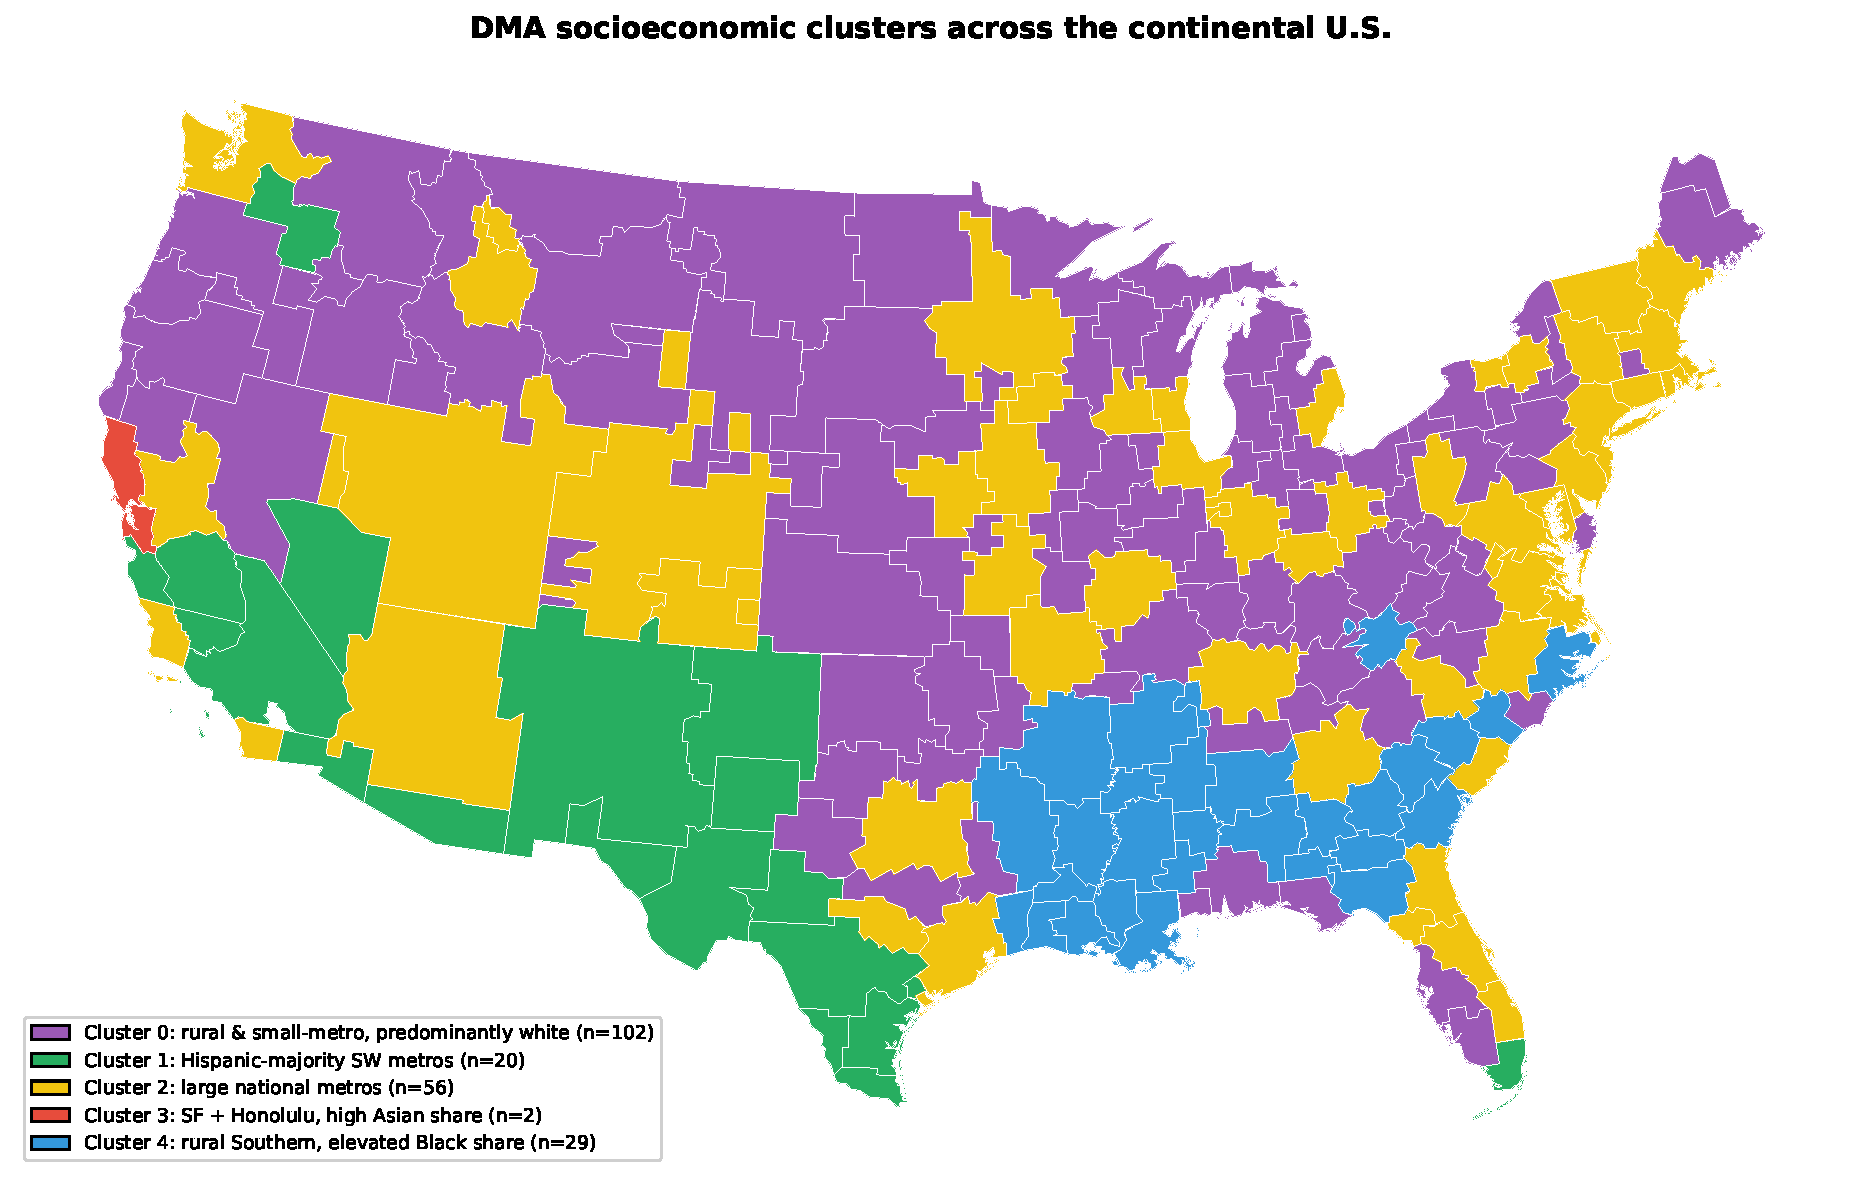
\includegraphics[width=0.95\linewidth]{../figures/fig_cluster_map.pdf}
\caption{Geographic distribution of the five DMA clusters across the continental U.S.\ (Hawaii and Alaska excluded). Cluster 4 (rural Southern, blue) tracks the historically defined Black Belt of the rural South~\citep{wimberley2002}; Cluster 1 (Hispanic-majority SW metros, green) traces the U.S.--Mexico border region and Southern California; Cluster 0 (rural and small-metropolitan, purple) is concentrated in the Midwest, Appalachia, the Plains, and the Pacific Northwest; and Cluster 2 (large national metros, yellow) marks coastal and inland metropolitan regions across the country.}
\label{fig:map}
\end{figure}

\begin{figure}[!htbp]
\centering
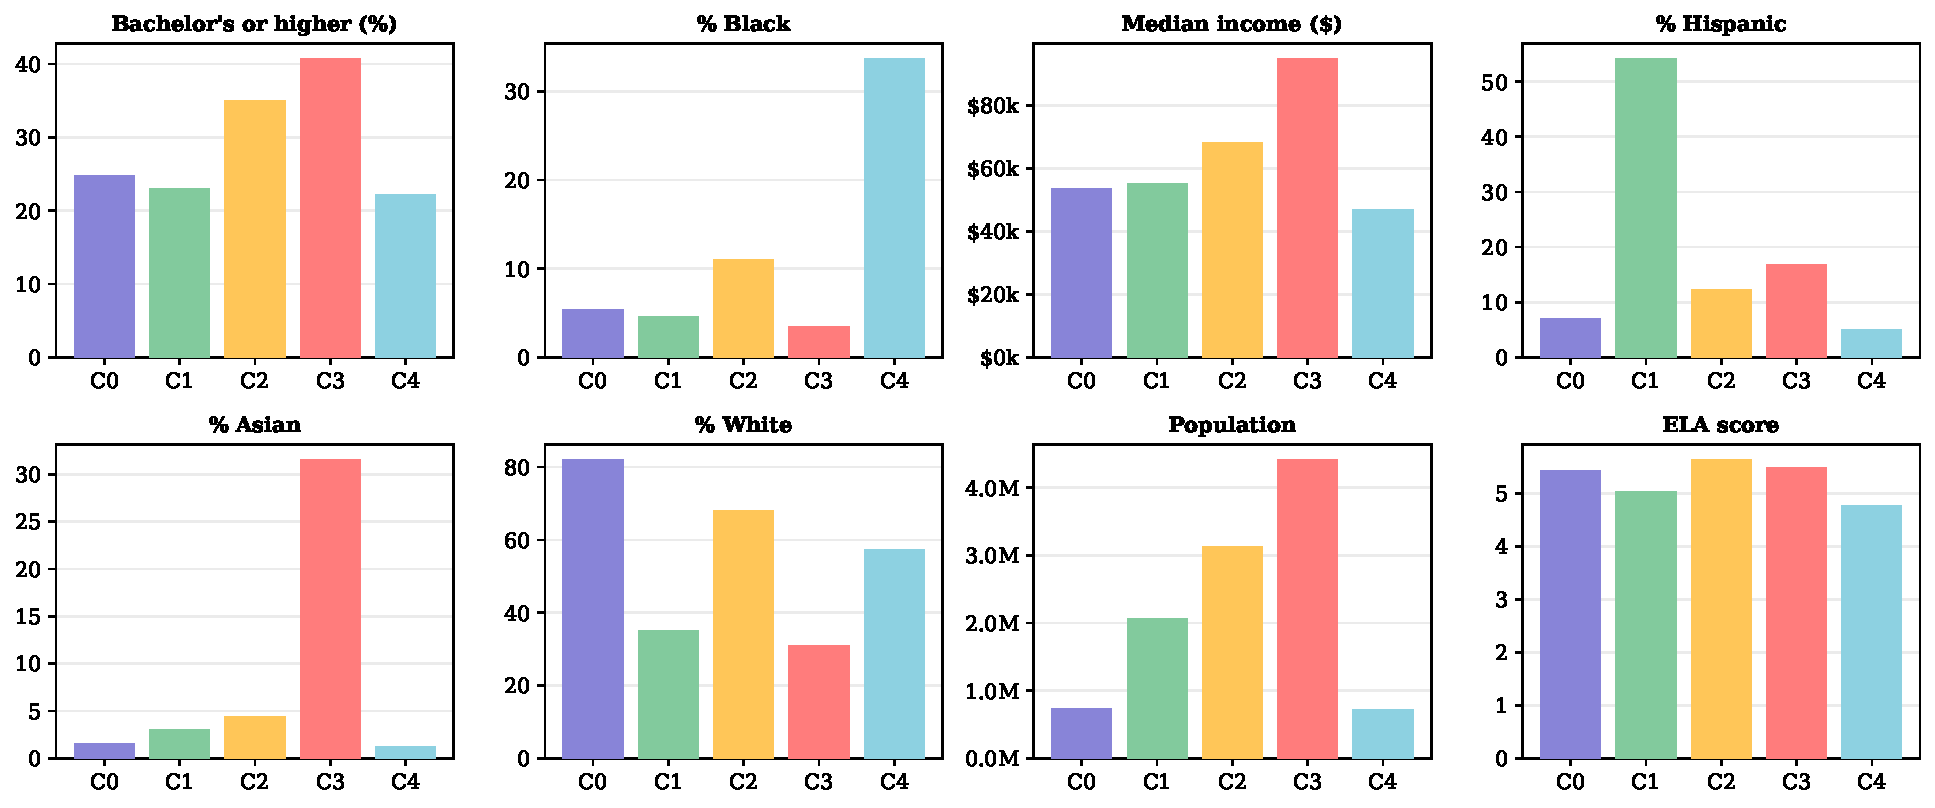
\includegraphics[width=\linewidth]{../figures/fig_cluster_bars.pdf}
\caption{Cluster means on the eight variables used to define the k-means typology.}
\label{fig:clusterbars}
\end{figure}

\begin{figure}[!htbp]
\centering
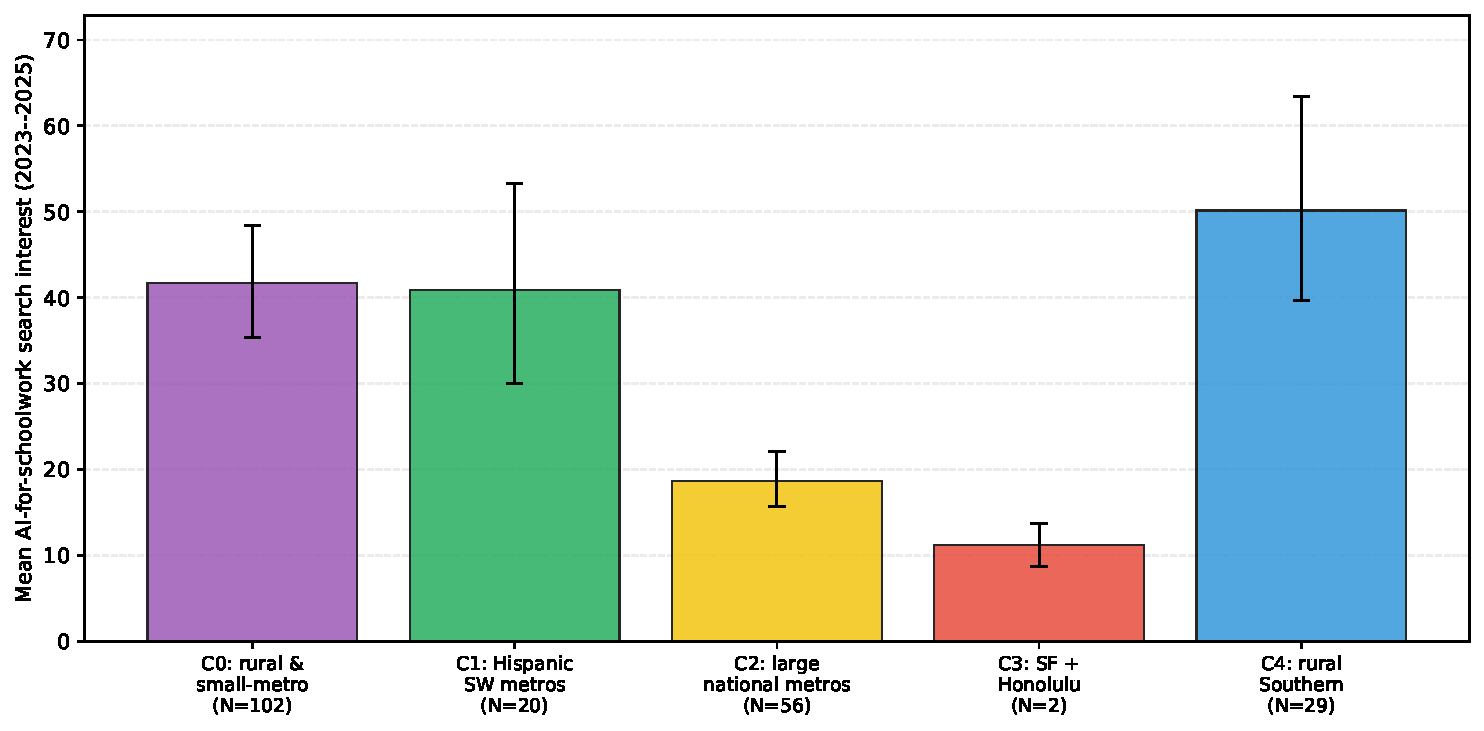
\includegraphics[width=0.85\linewidth]{../figures/fig_cluster_interest.pdf}
\caption{Mean 2023--2025 AI-for-schoolwork search interest by cluster, with 95\% bootstrap confidence intervals (2{,}000 resamples). The ranking inverts the regional pattern documented for general-purpose ChatGPT search interest by \citet{daepp2025}, in which higher-income, more-educated, and disproportionately Asian-American regions show the highest interest: here the affluent large-metro cluster (Cluster~2) and the small high-Asian-share metro pair (Cluster~3) show the lowest mean schoolwork-related search interest, while the three lower-income clusters (C0, C1, C4) show the highest.}
\label{fig:clusterinterest}
\end{figure}

\FloatBarrier
\subsection{Supervised prediction}
\label{sec:supervised}

We compared five regressors on the seven-feature supervised predictor set using repeated cross-validation (Table~\ref{tab:models}). Tree ensembles clearly outperform the linear family. Under 10 repetitions of 5-fold cross-validation with grid-searched hyperparameters, the tuned gradient boosting model achieves mean $R^2 = 0.39$ (SD 0.11 across the 50 folds, with per-repetition means ranging from 0.29 to 0.47) and a mean absolute error of $\approx 15.6$ search-interest points. We use repeated rather than single-split cross-validation because at $n=198$ a single fold assignment is unstable. Appendix~\ref{sec:approbust} reports the spread across repetitions and across alternative analytic samples.

We take the repeated-CV $R^2 \approx 0.39$ as the headline. It comfortably exceeds the $R^2 \approx 0.15$ ceiling of any linear model on the same features, and it is respectable given the small sample ($n=198$) and the measurement limits of both Google Trends and county-level ACS/SEDA aggregates. An untuned random forest attains a marginally higher mean ($R^2 = 0.42$) but with more than double the dispersion (SD 0.26 against 0.11). We therefore retain the tuned gradient boosting model as the headline on the basis of stability rather than mean alone. The qualitative story, that pre-existing disadvantage predicts subsequent student AI-for-schoolwork interest, is the same under every specification we examined.

\begin{table}[!htbp]
\centering
\small
\begin{tabular}{lrrr}
\toprule
Model & CV $R^2$ mean & CV $R^2$ SD & CV MAE \\
\midrule
Random Forest             & 0.418 & 0.259 & 13.1 \\
Gradient Boost (tuned)    & 0.388 & 0.112 & 15.6 \\
Gradient Boost (default)  & 0.315 & 0.362 & 14.2 \\
Lasso                     & 0.167 & 0.148 & 19.7 \\
Ridge                     & 0.151 & 0.183 & 19.8 \\
Linear                    & 0.150 & 0.184 & 19.8 \\
\bottomrule
\end{tabular}
\caption{Cross-validated performance (10 repetitions of 5-fold cross-validation, \texttt{random\_state=42}) of five regressors on the final seven-feature supervised predictor set (\texttt{median\_income}, \texttt{bach\_plus\_rate}, \texttt{population}, \texttt{pct\_hispanic}, \texttt{pct\_nh\_black}, \texttt{pct\_nh\_asian}, \texttt{score\_all\_ela}), estimated on the 198 DMAs with observed search interest. SD is taken across all 50 folds. The untuned random forest attains a marginally higher mean than the tuned gradient boosting model but with more than double the dispersion; the tuned gradient boosting model (grid search over \texttt{n\_estimators} $\in\{100,200,300\}$, \texttt{learning\_rate} $\in\{0.01,0.1,0.2\}$, \texttt{max\_depth} $\in\{3,5,7\}$, \texttt{min\_samples\_split} $\in\{2,5\}$) is the reported headline model.}
\label{tab:models}
\end{table}

Feature importance in the final gradient boosting model (Figure~\ref{fig:importance}) is distributed across population, bachelor-plus rate, income, racial composition, and ELA score, consistent with the feature-selection stage.

\begin{figure}[!htbp]
\centering
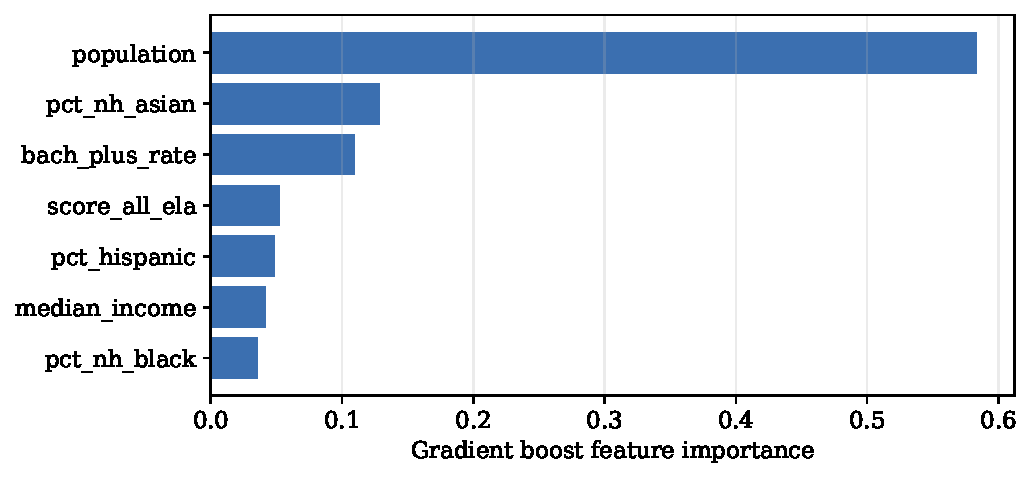
\includegraphics[width=0.85\linewidth]{../figures/fig_feature_importance.pdf}
\caption{Gradient boost feature importance (tree-based) in the tuned seven-feature model.}
\label{fig:importance}
\end{figure}

Figure~\ref{fig:obspred} plots cross-validated predictions against observed search interest. Calibration is good in the central range; the model slightly compresses the tails, under-predicting the highest-interest DMAs and over-predicting the lowest.

\begin{figure}[!htbp]
\centering
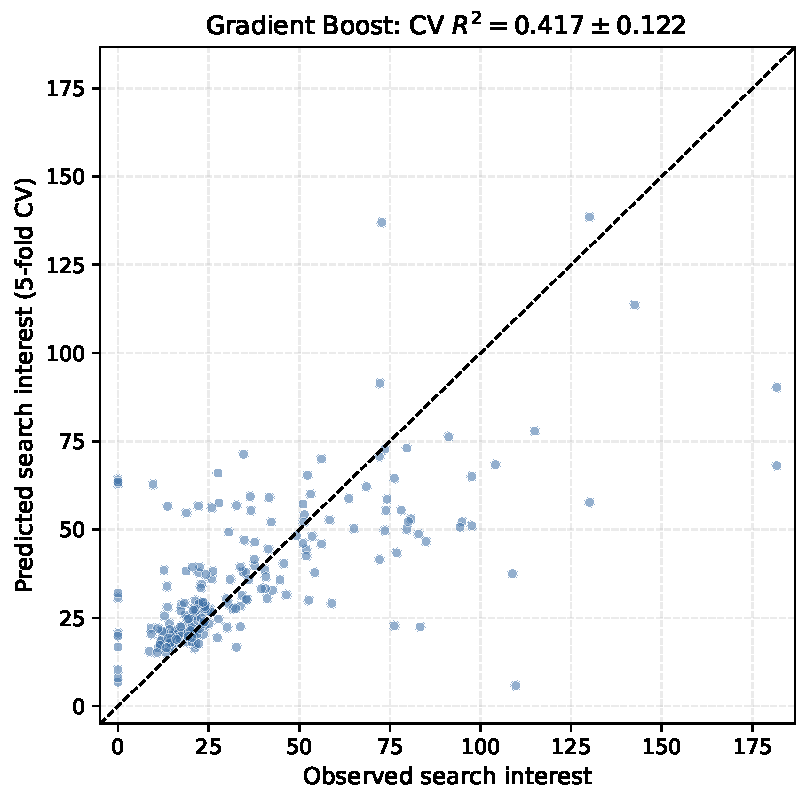
\includegraphics[width=0.55\linewidth]{../figures/fig_obs_pred.pdf}
\caption{Observed vs. 5-fold cross-validated predicted search interest from the tuned gradient boosting model. Dashed line is $y = x$.}
\label{fig:obspred}
\end{figure}

\FloatBarrier
% ==========================================================
\section{Discussion}

The central empirical finding---that pre-existing disadvantage predicts higher subsequent student AI-for-schoolwork search interest---fits uneasily with a simple digital-divide account. General-purpose ChatGPT awareness appears higher in more advantaged regions, but student-intent schoolwork search interest is higher in lower-income and less-educated regions. This divergence is consistent with recent student-level survey evidence showing elevated schoolwork-related chatbot use among Black and Hispanic teens~\citep{sidoti2025, pew2026}. The result suggests that the geography of student AI demand may differ from the geography of general AI awareness.

At least three interpretations are consistent with the regional pattern, and the present design cannot adjudicate between them.

\paragraph{Access-seeking.} Students in under-resourced communities may turn to generative AI as a low-cost substitute for scarce academic support such as tutoring, writing feedback, explanation, translation, test preparation, or homework help. Under this interpretation, high search interest is a signal of unmet educational demand, and the regional pattern reflects compensatory help-seeking by students whose schools and households cannot otherwise provide that support~\citep{sidoti2025, pew2026, zhang2025}.

\paragraph{Disengagement or assignment automation.} Students in under-resourced schools may be especially likely to search for AI tools as a shortcut through assignments they experience as alienating, low-value, or poorly supported. Under this interpretation, high search interest still signals a resource gap but reflects students attempting to bypass academic work rather than to engage with it. The two interpretations differ sharply in their implications for learning, but both point to the same structural fact: high-interest regions are regions where schools and households likely had fewer educational resources before ChatGPT.

\paragraph{Non-student traffic in student-intent keywords.} A third interpretation, which is in tension with the framing of the outcome but should be acknowledged, is that some search interest in our keyword set may be generated by parents searching on behalf of students, by teachers and administrators researching how to detect or respond to AI use, or by ESL learners using ``schoolwork''-coded queries to locate translation and explanation tools rather than to automate assignments. Each of these alternative populations could plausibly be larger in lower-income or higher-Hispanic regions for reasons unrelated to student demand per se. Our outcome cannot distinguish among searcher populations, and the magnitude of non-student traffic in student-intent keywords is unknown. We treat this as a real measurement-model uncertainty rather than a fatal flaw, as even if a substantial fraction of the signal is non-student, the policy implications below still apply to school-level responses, and survey evidence cited above documents elevated student-level use that is consistent with the regional pattern.

A punitive enforcement regime, including blanket bans, surveillance, and AI-detector-driven discipline, risks compounding existing inequities under all three interpretations. AI-detection tools are known to produce biased results against non-native-English speakers~\citep{liang2023, woelfel2023}, and Black students are already substantially more likely than white students to face exclusionary discipline of all kinds~\citep{darlinghammond2024}. This does not mean schools should ignore academic integrity. It means they should avoid treating AI use primarily as an individual misconduct problem when the strongest regional signal appears tied to structural disadvantage. A more productive policy stance would combine clear assignment-level rules, school-provided tools with transparent privacy and integrity settings, AI-literacy instruction, and assessment designs that reduce incentives for undisclosed automation while preserving legitimate support uses.

The regional concentration of demand has a further implication that the school-level recommendations above do not capture. Because student AI search interest is concentrated at the regional rather than the school level, AI policy is most coherent when it is also designed regionally---at the district, state-education-agency, or DMA level---rather than left to individual school administrators to negotiate in isolation. A district-level policy that pairs school-provided AI tools with shared assessment-design guidance, AI-literacy curricula, and consistent integrity standards across schools serving the same student-demand profile is likely to be both more equitable and more effective than school-by-school improvisation. This is a sharper policy claim that follows directly from the regional design used here: the unit at which the demand signal is meaningful (the DMA) is not the unit at which most AI policy is currently being made (the individual school).

% ==========================================================
\section{Limitations}

\paragraph{Choice of 2019 baseline.} We use 2019 because it is the last fully pre-COVID, pre-ChatGPT school year. Newer SEDA and Education Recovery releases provide valuable post-pandemic measures, but using 2021--2024 achievement data would change the estimand, as the predictors would partly reflect pandemic disruption and recovery rather than pre-existing regional conditions.

\paragraph{Interest is not usage.} Google Trends captures information-seeking, not tool use. High search interest for ``AI homework helper'' does not mean students in that DMA are using AI homework helpers, only that they are searching for them. We make no claims about usage rates. Interest is nonetheless a meaningful outcome on its own, as it reflects what students are looking for, which is an upstream signal of what tools they would use if barriers to access were removed.

\paragraph{Interest is not benefit.} Even if search interest reflects genuine demand for academic support, it does not show that students receive high-quality support or benefit educationally from AI. Prior research suggests that AI access, AI literacy, type of use, trust, and institutional guidance all shape whether students convert AI use into learning gains~\citep{zhang2025, zhang2026, beckman2025, yu2024}. This study therefore identifies where interest is concentrated, not whether generative AI narrows or widens achievement gaps in those places.

\paragraph{Google Trends reliability.} Google Trends scores are normalized, rounded, thresholded, and may vary across repeated pulls~\citep{holzl2025, googletrends}. The anchor-term strategy improves comparability across keyword batches but cannot eliminate all measurement error.

\paragraph{Multicollinearity.} The predictor set includes racial-proportion features that approach a compositional constraint (the four shares we use sum close to 100\% but not exactly, since smaller categories are excluded), along with correlated socioeconomic features (income, poverty, education). VIF values for the seven supervised features are reported in Appendix~\ref{sec:appimport} (Table~\ref{tab:vif}); all are below the conventional threshold of 5. The bootstrap Lasso further establishes that the \emph{set} of predictors is jointly stable and predictive. We therefore claim predictability of the outcome from the joint feature set without claiming identification of per-feature causal effects.

% ==========================================================
\section{Conclusion}

We asked what pre-ChatGPT regional conditions predict 2023--2025 student-intent search interest in AI for schoolwork. The answer is: smaller, lower-income, less-educated DMAs, which is an inversion of the usual ``technology adoption tracks advantage'' story and a divergence from the general-purpose ChatGPT search divide documented in prior regional work. Racial composition tracks this pattern regionally, in that the top-ranked cluster is a non-metropolitan Southern group with markedly elevated Black population shares, but it is not an independent predictor of interest in its own right. A gradient-boosting model on seven 2019 features explains about 39\% of the cross-region variance in post-ChatGPT student AI-for-schoolwork search interest under repeated cross-validation. The regional signal reported here is that places with smaller populations, lower income, and lower educational attainment show greater search interest in AI for schoolwork. That signal is distinct from, and independently corroborated by, student-level survey evidence showing elevated schoolwork-related chatbot use among Black and Hispanic teens. Because the present design is ecological, the survey evidence carries the individual-level claim, while this study carries the geographic one. The findings do not identify why, but they narrow the set of plausible explanations, from which we highlight three (access-seeking, disengagement, and non-student traffic), all of which have the same policy implication. That is, we should treat student AI interest as a signal of resource gaps, not as misconduct to be policed, and resist blanket punitive responses that will fall hardest on the communities most motivated to use the tools.

\paragraph{Future work.} Several extensions stand out. First, linking interest to actual usage---for example, via telemetry from school-sponsored AI tools, or via cross-walk to school-district-level survey data---would disambiguate the three interpretations and quantify the share of search interest attributable to students themselves rather than to parents, teachers, or other adult populations. Second, qualitative fieldwork in representative high- and low-interest DMAs would surface mechanisms (e.g., school AI policy, household device access, parental supervision) that quantitative signals cannot. Third, a longitudinal version of this study run annually would show whether the inverse relationship stabilizes, attenuates, or flips as generative AI diffuses further. Fourth, a more granular keyword decomposition (separating academic-integrity terms from help-seeking terms from school-policy terms) would test whether the regional pattern is driven primarily by help-seeking, by enforcement concern, or by both.

% ==========================================================
\section*{Code and data availability}
Code, the processed dataset, and a reproducible analysis notebook are archived
in a public repository with a permanent DOI. The repository URL and DOI are
withheld here to preserve anonymity during review, and will be given in the
camera-ready version. Raw Google Trends responses are provided as CSVs; Trends
queries are not guaranteed to replicate exactly over time because the
underlying API is non-deterministic.

% ==========================================================
\bibliographystyle{aaai25}
\bibliography{../refs}

% ==========================================================
\appendix
\section{Full keyword list and batch assignments}
\label{sec:appkeywords}

The 19 batches of five keywords each are reproduced below exactly as queried, with the anchor ``homework'' appearing in every batch:

\begin{enumerate}
\item homework, AI biology homework, PhotoMath alternatives, AI foreign language homework, homework prompts for AI
\item homework, AI for writing essays, how to prompt AI for homework, Socratic app homework, AI flashcards
\item homework, AI for literature review, Best AI prompts for homework, AI homework helper app, Academic integrity AI
\item homework, AI plagiarism risk, AI practice problems, AI homework answers wrong, how accurate are AI detectors
\item homework, AI for group projects, AI for high school, Is Claude allowed for school?, AI to generate discussion questions
\item homework, AI for language learning homework, Gemini homework help, Is ChatGPT allowed for school?, AI study techniques
\item homework, paraphrasing tool to avoid plagiarism, AI to summarize textbooks, is using AI cheating, AI homework Discord bot
\item homework, how to avoid AI detection, AI for math problems, AI for studying, AI prompt engineering for school
\item homework, can teachers detect AI, AI for book report, Turnitin AI detection, School policy on AI
\item homework, AI essay writer, AI economics help, how to cite AI, AI calculus solver
\item homework, AI English essay, Khanmigo, bypass AI checker, AI chemistry homework
\item homework, ChatGPT for homework, AI citation generator, AI for lab report, AI hallucination homework
\item homework, how to fact-check AI homework, make AI undetectable, AI for college students, AI for studying for tests
\item homework, is using QuillBot plagiarism, AI for exam prep, AI history essay help, AI homework inaccuracies
\item homework, University AI policy, AI for presentation outline, when AI gets homework wrong, AI learning assistant
\item homework, Is Gemini allowed for school?, AI homework solver, Claude for homework, AI homework help
\item homework, AI statistics solver, AI physics problems, homework AI app, PhotoMath
\item homework, how to use AI for research, AI homework mistakes, QuillBot for school, Copilot for students
\item homework, AI tutor app
\end{enumerate}

\section{Data dictionary}
\label{sec:appdata}

\begin{table}[!htbp]
\centering
\small
\begin{tabular}{lll}
\toprule
Variable & Source & Description \\
\midrule
\texttt{search\_interest}    & Google Trends & Anchor-normalized mean over 73 target keywords, 2023--2025 \\
\texttt{median\_income}      & ACS5 2019    & Population-weighted DMA median household income \\
\texttt{poverty\_rate}       & ACS5 2019    & Share below federal poverty line \\
\texttt{bach\_plus\_rate}    & ACS5 2019    & Share of adults with bachelor's or higher \\
\texttt{grad\_prof\_rate}    & ACS5 2019    & Share with master's, professional, or doctoral \\
\texttt{population}          & ACS5 2019    & Total DMA population \\
\texttt{pct\_hispanic}       & ACS5 2019    & Hispanic or Latino share (any race) \\
\texttt{pct\_nh\_white}      & ACS5 2019    & Non-Hispanic white share \\
\texttt{pct\_nh\_black}      & ACS5 2019    & Non-Hispanic Black share \\
\texttt{pct\_nh\_asian}      & ACS5 2019    & Non-Hispanic Asian share \\
\texttt{score\_all\_ela}     & SEDA 2019    & Mean ELA score across tested grades \\
\texttt{score\_all\_math}    & SEDA 2019    & Mean math score across tested grades \\
\bottomrule
\end{tabular}
\caption{Variables used in the final model. Rates are population-weighted from county to DMA; SEDA scores are weighted by total assessments.}
\label{tab:vars}
\end{table}

\section{Cluster geography and demographic verification}
\label{sec:appclusters}

Table~\ref{tab:clusterverify} reports the empirical evidence underpinning the cluster characterizations in Section~5.3. State distributions are computed from the trailing two-letter state code in each DMA name; Southern share is the proportion of cluster-member DMAs whose state code is in \{AL, AR, FL, GA, KY, LA, MS, NC, OK, SC, TN, TX, VA, WV\}; racial-share columns are population-weighted means of the underlying ACS5 2019 county-level shares.

\begin{table}[!htbp]
\centering
\small
\begin{tabular}{lrrrrrr}
\toprule
Cluster & N & Top represented states (count) & South share & \% White & \% Black & \% Hispanic \\
\midrule
0 & 102 & OH(7), MI(6), NY(5), IL(5), OR(4), MT(4), WV(4) & 28\% & 82.1 & 5.4 & 7.0 \\
1 & \phantom{0}20 & TX(10), CA(5), NM(1), NV(1), FL(1), AZ(1), WA(1) & 55\% & 35.1 & 4.6 & 54.2 \\
2 & \phantom{0}56 & NY(5), FL(4), AK(3), TX(3), VA(3), MO(3), CA(3) & 27\% & 68.1 & 11.0 & 12.3 \\
3 & \phantom{00}2 & HI(1), CA(1) & \phantom{0}0\% & 30.9 & 3.5 & 16.9 \\
4 & \phantom{0}29 & GA(6), LA(6), MS(5), AL(3), SC(2), TN(2), AR(2) & 97\% & 57.4 & 33.7 & 5.0 \\
\bottomrule
\end{tabular}
\caption{Empirical verification of cluster labels: state distributions, Southern-state share, and racial-composition means. Cluster~4's near-total concentration in former Confederate states with markedly elevated Black population shares supports the Black-Belt-region characterization in Section~5.3 and Figure~\ref{fig:map}; Cluster~1's concentration in Texas and California supports the Hispanic-majority Southwestern-metros characterization; Cluster~0's representation in OH, MI, IL, NY, OR, MT, and WV supports the mid-size predominantly-white characterization across the Midwest, Plains, and Pacific Northwest.}
\label{tab:clusterverify}
\end{table}

\section{Variance inflation factors}
\label{sec:appimport}

Table~\ref{tab:vif} reports variance inflation factors for the seven supervised features on $z$-scored predictors. All values are below the conventional threshold of 5; \texttt{median\_income} and \texttt{bach\_plus\_rate} are the most collinear pair (consistent with the well-known income--education association), but neither rises to the level at which mechanical confounding would be expected. We therefore take the joint feature set as identifiable in the supervised model.

\begin{table}[!htbp]
\centering
\small
\begin{tabular}{lr}
\toprule
Feature & VIF \\
\midrule
\texttt{median\_income}    & 4.32 \\
\texttt{bach\_plus\_rate}  & 3.30 \\
\texttt{pct\_nh\_asian}    & 1.83 \\
\texttt{population}        & 1.70 \\
\texttt{pct\_nh\_black}    & 1.49 \\
\texttt{score\_all\_ela}   & 1.47 \\
\texttt{pct\_hispanic}     & 1.26 \\
\bottomrule
\end{tabular}
\caption{Variance inflation factors for the seven supervised features (z-scored, $n=198$). All values are below the conventional VIF threshold of 5.}
\label{tab:vif}
\end{table}

% ==========================================================
\section{Robustness to the treatment of missing outcomes and to influential observations}
\label{sec:approbust}

Section~\ref{sec:data} adopts the 198 DMAs with observed search interest as the primary analytic sample, and notes that the alternative treatment, coding the eleven unobserved DMAs at zero, errs in the opposite direction. Table~\ref{tab:robust} reports the tuned gradient boosting model under both treatments, together with two further sensitivity checks: dropping the smallest 20\% of DMAs by population, which addresses the concern that Google Trends is least reliable at low search volume, and winsorizing the outcome at its 99th percentile, which addresses the influence of the most extreme observed values.

\begin{table}[!htbp]
\centering
\small
\begin{tabular}{lrrr}
\toprule
Analytic sample & $N$ & $R^2$ mean (SD) & Per-repetition range \\
\midrule
Observed outcomes only (primary)      & 198 & 0.388 (0.112) & 0.294--0.474 \\
Unobserved outcomes coded at zero     & 209 & 0.352 (0.262) & 0.153--0.439 \\
Smallest 20\% of DMAs dropped         & 158 & 0.431 (0.202) & 0.317--0.556 \\
Outcome winsorized at 99th percentile & 198 & 0.415 (0.087) & 0.369--0.475 \\
\bottomrule
\end{tabular}
\caption{Tuned gradient boosting model under four analytic samples, each estimated with 10 repetitions of 5-fold cross-validation and re-tuned within its own sample. SD is taken across all 50 folds; the per-repetition range gives the smallest and largest of the ten repetition-level means.}
\label{tab:robust}
\end{table}

Three points follow. First, every alternative sample yields a mean $R^2$ at or above the primary specification except the deliberately conservative zero-coded sample, which is also by far the least stable (SD 0.262 against 0.112). Coding unobserved DMAs at the floor therefore adds variance rather than information, consistent with the argument in Section~\ref{sec:data} that it attenuates rather than inflates the reported gradient. Second, dropping the smallest DMAs \emph{strengthens} the fit, which is the opposite of what a low-volume Google Trends artifact would predict. Third, the cluster ordering reported in Section~\ref{sec:results} is identical under both outcome treatments, as are the sign and significance of every univariate gradient we report.

\end{document}